\section{Entradas flotantes en compuertas TTL y CMOS}
\vspace{5mm}
Se implementaron los siguientes circuitos:

\begin{figure}[H]
    \begin{minipage}{.49\linewidth}
        \centering
        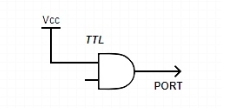
\includegraphics[width=.6\linewidth]{./TTLFlotante.jpg}
        \caption{Compuerta AND TTL con entrada flotante.}
        \label{fig:TTLFlotante}
    \end{minipage}
    \begin{minipage}{.5\linewidth}
        \centering
        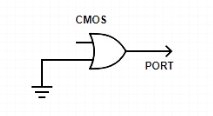
\includegraphics[width=.5\linewidth]{./CMOSFlotante.jpg}
        \caption{Compuerta OR CMOS con entrada flotante.}
        \label{fig:CMOSFlotante}
    \end{minipage}
\end{figure}

En primer lugar, en el caso de la compuerta TTL se conectó una entrada a Vcc (5V) y se dejó la otra flotante (figura \ref{fig:TTLFlotante}),
 es decir no se le realizó ninguna conexión y se midió la salida, que se observó constante como un 1 lógico (aproximadamente 5V). \\
En el caso de la CMOS, se dejó también un input flotante y otro se lo conectó a masa, como se ve en la figura \ref{fig:CMOSFlotante}. 
Se observó en este caso ruido de línea de 50Hz, con amplitud que variaba entre 0-0.8V, que no se encontraba entre las tensiones high y low de salida 
del CMOS ($V_{OH}~y~V_{OL}$)\footnote{Datos sacados de la datasheet: ver figura \ref{fig:cmos-threshold}.},
 es decir, la salida era indefinida (no era ni un 1 ni un 0 lógico). 

\begin{figure}[H]
    \centering
    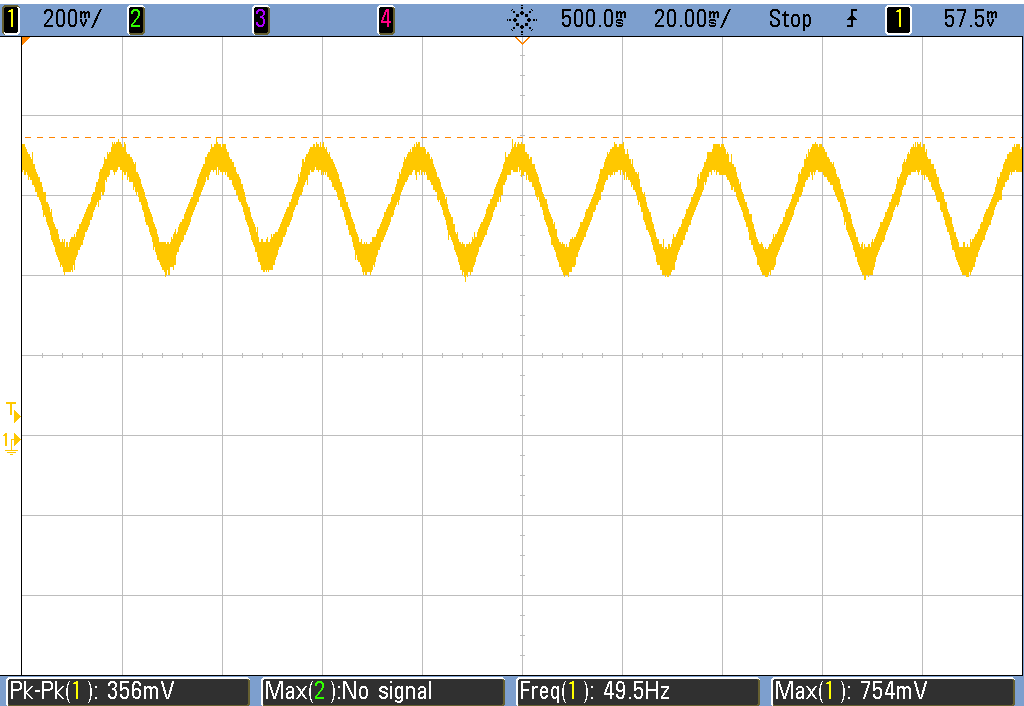
\includegraphics[width=.5\linewidth]{./ruidoCMOS.png}
    \caption{Ruido observado del CMOS con entrada flotante.}
    \label{fig:ruidoCMOS}
\end{figure}

\vspace{20mm}
\begin{wraptable}{l}{6.5cm}
    \begin{center}
        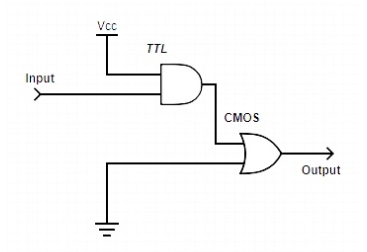
\includegraphics[scale=0.5]{./circuito.jpg}
        \caption{Circuito implementado.}
        \label{fig:circuito}
    \end{center}
\end{wraptable} 
\par
Para el CMOS este comportamiento puede deberse a que tienen altas impedancias de entrada por lo que al dejar una entrada flotante
funciona como antena, induciéndose corrientes, por ejemplo, por ruido, lo que genera tensiones a la entrada de la compuerta
ocasionando un nivel de tensión high o low incierto a la salida.
A continuación se implementó el circuito de la figura \ref{fig:circuito}. No se observó 



A floating TTL input usually acts as a HIGH input.
Es decir una entrada flotante en un TTL es considerada como un 1 lógico a la entrada.

//justificar con hoja de datos, que dice q hay q ponerla a vcc o ground(dependiendo esta eleccion de la funcion del cicuito), o sea tiene q ser una tension conocida
Ademas que al cmos, al dejarlo flotante se calienta el integrado porq le estas exigiendo (metiendo) mas corriente.
como que tira hasta 0.8v a la salida que segun la datasheet es basura (porq esta entre vol y voh que es 0.2-2.4, creo)

\begin{figure}[H]
    \begin{minipage}{.49\linewidth}
        \centering
       % \includegraphics[width=.6\linewidth]{./.jpg}
        \caption{Compuerta AND TTL con entrada flotante.}
        \label{fig:ttl-threshold}
    \end{minipage}
    \begin{minipage}{.5\linewidth}
        \centering
        %\includegraphics[width=.5\linewidth]{./.jpg}
        \caption{Compuerta OR CMOS con entrada flotante.}
        \label{fig:cmos-threshold}
    \end{minipage}
\end{figure}


, another solution is to connect unused inputs to an input of the same gate that is in use. The function of the device
is unaffected. This circuit arrangement can be used equally well with AND (NAND) as with OR (NOR) gates 
NOTA: seccion Unused Inputs http://www.ti.com/lit/an/sdya009c/sdya009c.pdf

%leer esto https://www.fairchildsemi.com/application-notes/AN/AN-363.pdf
leer tambien esto http://www.ti.com/lit/an/scba004d/scba004d.pdf

cuando le entro al  circuito con 1.4V sale cualquier cosa, como se puede ver en la figura "circuito sale mal" (tambien pasa con los dos LS asi q no se si chamuyar coon esto)
